% !TeX program = lualatex
% Report for the Intelligent Robot Manipulation project lab.
\documentclass[
  english,
  accentcolor=11b,
  type=intern,
  marginpar=false,
  logofile=figures/PEARLTUDA.png
]{tudapub}

\usepackage[main=english,ngerman]{babel}
\usepackage[autostyle]{csquotes}
\usepackage{booktabs}
\usepackage{graphicx}
\usepackage{microtype}
\usepackage{natbib}
\usepackage{tabularx}
\usepackage{array}
\usepackage{xcolor}
\usepackage{listings}
\usepackage{enumitem}
\usepackage{siunitx}
\usepackage[section]{placeins}
\usepackage{subcaption}
\usepackage{tikz}
\usetikzlibrary{positioning,arrows.meta,calc}
\usepackage{pgfplots}
\pgfplotsset{compat=1.18}

\definecolor{PearlBlue}{HTML}{00689D}
\definecolor{SoftBlue}{HTML}{EAF4F8}
\definecolor{SoftGray}{HTML}{F3F5F6}
\definecolor{TCGreen}{HTML}{1baf7a}
\definecolor{TCBlue}{HTML}{2a78d6}
\definecolor{TCOrange}{HTML}{eb6834}

% Perceptual-magma approximation for the clip-panel spectrograms (Section 6),
% so the pgfplots colorbar matches the embedded raster heatmaps.
\pgfplotsset{
  colormap={magma}{
    rgb255=(0,0,4) rgb255=(28,16,68) rgb255=(79,18,123) rgb255=(129,37,129)
    rgb255=(181,54,122) rgb255=(229,80,100) rgb255=(251,135,97)
    rgb255=(254,194,135) rgb255=(252,253,191)
  }
}

% Shared styling for the block diagrams in Section 4, so every figure in
% the report reads as one drawn system rather than three separate sketches.
\tikzset{
  diagbox/.style={draw=PearlBlue, semithick, rounded corners=1.5pt, align=center,
    inner xsep=7pt, inner ysep=5pt, minimum height=8.5mm, font=\sffamily\small},
  diagio/.style={diagbox, fill=white},
  diagproc/.style={diagbox, fill=PearlBlue!7},
  diagterm/.style={diagbox, fill=PearlBlue, text=white, draw=PearlBlue},
  diagarrow/.style={-{Latex[length=2.1mm,width=1.5mm]}, PearlBlue, semithick},
  diaglabel/.style={font=\sffamily\scriptsize, align=center, fill=white,
    inner sep=1.5pt, text=PearlBlue!85!black},
}

\hypersetup{
  colorlinks=true,
  linkcolor=PearlBlue,
  citecolor=PearlBlue,
  urlcolor=PearlBlue,
  pdftitle={Audio for Contact-Rich Manipulation},
  pdfauthor={Paolo Andoni}
}

\newcolumntype{Y}{>{\raggedright\arraybackslash}X}
\DeclareRobustCommand{\topic}[1]{\texttt{\detokenize{#1}}}
\DeclareRobustCommand{\rosnode}[1]{\texttt{\detokenize{#1}}}
\DeclareRobustCommand{\code}[1]{\texttt{\detokenize{#1}}}

\lstdefinestyle{terminal}{
  basicstyle=\ttfamily\small,
  backgroundcolor=\color{SoftGray},
  frame=single,
  rulecolor=\color{SoftGray},
  breaklines=true,
  columns=fullflexible,
  keepspaces=true,
  showstringspaces=false
}

\title{Audio for Contact-Rich Manipulation}
\author{Paolo Andoni\\Supervised by Rickmer Krohn}
\date{September 2026}

\begin{document}

\maketitle

\begin{abstract}
Cameras often miss what happens at the moment of contact: when a gripper wipes a table or pushes a peg into a hole, the contact itself is hidden by the gripper and the part. The sound of the contact can fill this gap. This project lays the groundwork for adding audio as a sensor to a robot that already uses vision and its own joint state.

Based on a review of the literature on audio in robot manipulation, a ROS~2 pipeline was built. It records audio, converts it into a log-mel spectrogram, encodes it with a neural network, and publishes the resulting features so that a policy can use them together with camera images and robot state. After recording, each piece of audio is matched with the robot's position at the same time, and the robot's actions are computed from its movement. This matching was tested with a simulated robot. First results are encouraging. In hand recordings made with an air microphone and substitute objects, a classifier using pretrained Audio Spectrogram Transformer features identified the correct sound category in 15 of 18 clips. These recordings support the planned cleaning and peg-insertion study. In an early test on a published contact-microphone dataset, audio features gave lower motion-prediction error than a constant baseline.

The next step is to mount a contact microphone on the gripper of the Franka arm, measure the robot's own noise, record teleoperated demonstrations, and compare policies trained with and without audio by their task success on the real robot.
\end{abstract}

\tableofcontents

\section{Literature Review}
\label{sec:lit}

This section groups the related work into four topics and then summarises what they have in common and what it means for this project.

\subsection{Sound as a sensor for manipulation}

Early work used sound to estimate things a camera sees poorly, such as the amount of granular material a robot scoops \citep{clarke2018granular} or the liquid height while pouring \citep{liang2019pouring}. \citet{gandhi2020swoosh} recorded 15,000 interactions of 60 objects on a tilting tray with contact microphones and showed that the sound alone identifies most objects and helps predict how they move. \citet{mejia2024hearing} use a contact microphone on the gripper as a tactile sensor. Because its signal is ordinary audio, an encoder pretrained on large audio-visual datasets can be reused, which is not possible for most tactile sensors.

\subsection{Combining sound with vision and touch}

\citet{li2022seehearfeel} fuse a camera, a contact microphone and a GelSight tactile sensor and show that they complement each other: vision gives the global scene, audio reports events immediately, and touch gives local geometry. \citet{du2022playbyear} learn audio-visual policies on a Franka Panda for tasks where the camera cannot see the important object, such as pulling keys out of a bag. \citet{lee2019visiontouch} study peg insertion with vision and force sensing and show that for insertion the contact signal carries the information the camera is missing.

\subsection{Learning manipulation from demonstrations}

Diffusion Policy \citep{chi2023diffusion} and ACT \citep{zhao2023act} learn from demonstrations and predict a chunk of future actions instead of a single step. The Universal Manipulation Interface (UMI) \citep{chi2024umi} is a handheld gripper with a camera for collecting such demonstrations without a robot. ManiWAV \citep{liu2024maniwav} adds a contact microphone to the UMI finger and trains a diffusion policy on images, audio and pose for tasks such as wiping and pouring. It also shows a practical problem: on the robot, motor noise changes the audio compared with the handheld demonstrations. The authors reduce this gap by mixing recorded robot noise and background sounds from ESC-50 \citep{piczak2015esc} into the training audio.

\subsection{Audio representations}

The Audio Spectrogram Transformer (AST) \citep{gong2021ast} is the encoder used by ManiWAV and in this project. It cuts a log-mel spectrogram into patches, like an image, and processes them with a Transformer. This project uses weights pretrained on AudioSet \citep{gemmeke2017audioset}, a large collection of everyday sounds, while ManiWAV trains its AST from scratch. Augmentation such as SpecAugment \citep{park2019specaugment} makes such models more robust to new recording conditions.

\subsection{General points and relation to this project}
\label{sec:lit-points}

Four points appear across these works, and each shaped a decision in this project.

\begin{enumerate}[leftmargin=*,label=\textbf{P\arabic*:},itemsep=4pt]
  \item \textbf{Sound helps where the camera cannot see}, for example at a contact hidden by the gripper. This is why cleaning and peg insertion were chosen as tasks (Section~\ref{sec:choosing-task}).
  \item \textbf{The robot works use contact microphones.} The recordings in this project used an air microphone (Section~\ref{sec:pipeline}), so a contact microphone is the first hardware step for the robot experiment.
  \item \textbf{Audio is added to vision and robot state, not used instead of them}, and policies use a short history to predict chunks of actions. The pipeline therefore publishes audio features for a policy and prepares action chunks based on the recorded poses (Section~\ref{sec:policy-data}).
  \item \textbf{Timing and robot noise are the practical problems.} Every message in the pipeline carries its capture time (Section~\ref{sec:alignment}), and robot noise is discussed in Section~\ref{sec:robot-noise}.
\end{enumerate}

\section{Motivation and Research Questions}

The robot in this project already uses vision and its joint state. The goal is to prepare contact audio as an additional input for this robot, because in contact-rich tasks the camera often does not show clearly what happens when the robot touches an object or a surface. This leads to two research questions:

\begin{enumerate}[leftmargin=*,label=\textbf{RQ\arabic*:},itemsep=7pt]
  \item Can contact audio provide task-relevant information about contact events, object state, or material when vision and robot proprioception are ambiguous or incomplete?
  \item Can contact audio be acquired, represented, and time-aligned in ROS~2 reliably enough to serve as an input to a robot policy alongside vision and robot state?
\end{enumerate}

RQ1 can only be answered on the real robot, by comparing policies with and without audio. RQ2 is the engineering question addressed by the software in this project, which prepares that experiment.

\section{Project Scope}

The idea of this project is an experiment on the real robot: does a policy that hears its contact sounds perform better than one that only sees? To prepare it, the project covers five parts:

\begin{enumerate}[leftmargin=*]
  \item acquire live microphone audio, or replay a WAV file through the same interface;
  \item transform the waveform into a documented log-mel spectrogram;
  \item publish the spectrogram in ROS~2 and encode it into features in a separate ML node;
  \item keep the capture timestamps and align the audio windows offline with \topic{/joint_states}, \topic{/tf}, and camera data;
  \item assemble the observations a policy consumes and derive the matching actions from the recorded trajectories.
\end{enumerate}

\section{From Audio Waveform to a ROS 2 Pipeline}
\label{sec:pipeline}

This section describes the software built in this project. It explains how the audio signal is represented, how the processing is split into two ROS~2 \citep{macenski2022ros2} nodes, how the robot state is aligned with the audio, and how observations and actions for a policy are produced. Because two different kinds of microphone appear in this report, the section starts with the sensor.

\paragraph{Contact microphone and air microphone.} A \emph{contact microphone}, as used in the robot works of Section~\ref{sec:lit}, is a piezoelectric element attached to a solid part such as a gripper finger; it measures the vibrations travelling through that part. The recordings in this project were made with an ordinary \emph{air microphone}, a USB condenser microphone placed close to the contact point, which also picks up the noise in the room. The software works with both, but the signals differ, so results from the air microphone do not transfer directly to a contact microphone.

\subsection{The audio representation}

The microphone produces a waveform that describes air pressure (air microphone) or structural vibration (contact microphone) over time. An audio encoder needs a more compact view of this signal, so the waveform is converted into a spectrogram that shows how its frequencies change over time. The implemented preprocessing path is shown in Figure~\ref{fig:audio-chain}.

\begin{figure}[htbp]
  \centering
  \resizebox{\textwidth}{!}{%
  \begin{tikzpicture}[node distance=5mm, >=Latex]
  \node[diagio]                    (wav)    {Waveform};
  \node[diagproc, right=of wav]    (resamp) {Resampling\\\footnotesize\SI{16}{kHz}};
  \node[diagproc, right=of resamp] (stft)   {Short-time\\Fourier transform};
  \node[diagproc, right=of stft]   (mel)    {Mel\\filterbank};
  \node[diagproc, right=of mel]    (log)    {Logarithmic\\scaling};
  \node[diagterm, right=of log]    (spec)   {Spectrogram\\message};
  \foreach \a/\b in {wav/resamp, resamp/stft, stft/mel, mel/log, log/spec}
    \draw[diagarrow] (\a) -- (\b);
  \end{tikzpicture}%
  }
  \caption{The implemented audio preprocessing chain, from the raw waveform to the spectrogram message published on the ROS~2 topic.}
  \label{fig:audio-chain}
\end{figure}

Audio is resampled to \SI{16}{kHz}. A \SI{25}{ms} analysis frame and a \SI{10}{ms} frame shift give 98 time frames for a one-second buffer, each with 128 mel-frequency bins. The resulting $98\times128$ filterbank is published without the padding that AST needs. This keeps the ROS message small and puts model-specific padding and normalisation into the model that requires them.

\begin{figure}[htbp]
  \centering
  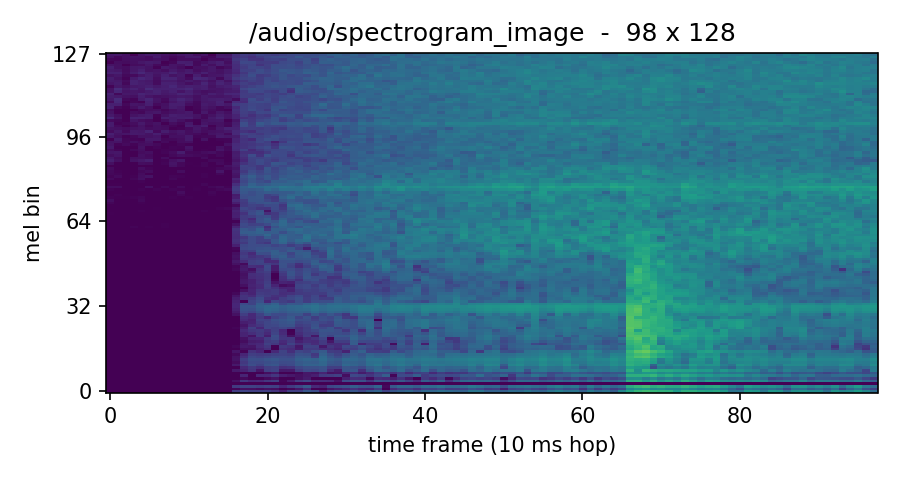
\includegraphics[width=0.68\textwidth]{figures/spectrogram_example.png}
  \caption{Actual image published by the pipeline for a one-second audio window. The horizontal axis contains 98 time frames and the vertical axis contains 128 mel-frequency bins. This is the same unpadded log-mel representation sent to the ML node; it is not an evaluation result.}
  \label{fig:spectrogram}
\end{figure}

\subsection{Two nodes}

The pipeline consists of two main nodes (Figure~\ref{fig:pipeline}). The \rosnode{audio_daq_node} handles everything close to the sensor: capture, buffering, resampling, filterbank computation and publication. It accepts either a live microphone or a WAV file, so the same interface works during development and in the lab.

The \rosnode{contact_ml_node} subscribes to \topic{/audio/spectrogram} and passes it through an encoder. It publishes the resulting embedding on \topic{/audio/embedding} and the predicted class on \topic{/audio/contact_prediction}. Different encoders can be tried in this node. AST was used as the main encoder, because it is the one used in the literature, but smaller encoders can also be trained from scratch. Two of them are compared with AST in Section~\ref{sec:separation}: a small convolutional network (CNN) and simple statistics over the mel bands (\code{melstats}), which need no neural network. Since the audio processing happens in the other node, changing the encoder does not change the spectrogram.

\begin{figure}[htbp]
  \centering
  \resizebox{\textwidth}{!}{%
  \begin{tikzpicture}[node distance=9mm and 12mm, >=Latex,
    nodetitle/.style={draw=none, font=\sffamily\bfseries\small, text=PearlBlue, inner sep=0pt}
  ]
  \node[diagio] (mic) {Microphone};
  \node[diagio, below=11mm of mic] (wav) {WAV file};

  \node[diagproc, right=30mm of mic, yshift=-5.5mm, text width=3.7cm,
        align=left, inner ysep=9mm] (daq)
    {Capture\\ Buffering\\ Resampling\\ Filterbank construction\\ Publication};
  \node[nodetitle] at ($(daq.north)+(0,-3.6mm)$) {\texttt{audio\_daq\_node}};
  \draw[PearlBlue!55] ([yshift=-6.2mm]daq.north west) -- ([yshift=-6.2mm]daq.north east);

  \node[diagproc, right=38mm of daq, text width=3.6cm,
        align=left, inner ysep=9mm] (ml)
    {Spectrogram decoding\\ Encoding (interchangeable)\\ Classification};
  \node[nodetitle] at ($(ml.north)+(0,-3.6mm)$) {\texttt{contact\_ml\_node}};
  \draw[PearlBlue!55] ([yshift=-6.2mm]ml.north west) -- ([yshift=-6.2mm]ml.north east);

  \node[diagterm, right=26mm of ml, yshift=11mm] (pred) {\topic{/audio/contact_prediction}};
  \node[diagterm, right=26mm of ml, yshift=-11mm] (embed) {\topic{/audio/embedding}};

  \draw[diagarrow] (mic) -- (daq);
  \draw[diagarrow] (wav) -- (daq);
  \draw[diagarrow] (daq) -- node[diaglabel, above] {\topic{/audio/spectrogram}} (ml);
  \draw[diagarrow] (ml) -- (pred);
  \draw[diagarrow] (ml) -- (embed);
  \end{tikzpicture}%
  }
  \caption{The implemented ROS~2 audio subsystem. Acquisition and representation belong to the DAQ node; encoding and classification belong to the ML node.}
  \label{fig:pipeline}
\end{figure}

\subsection{Where robot state enters}
\label{sec:alignment}

The robot's joint positions come from the robot driver, not from the audio pipeline. During an experiment, the audio, the joint positions and the camera images are all recorded into one ROS~2 bag (Figure~\ref{fig:alignment-flow}).

\begin{figure}[htbp]
  \centering
  \resizebox{\textwidth}{!}{%
  \begin{tikzpicture}[>=Latex]
  \node[diagio]                        (mic)   at (0,4.2)    {Microphone};
  \node[diagproc]                      (daq)   at (4.2,4.2)  {\texttt{audio\_daq\_node}};
  \node[diagproc]                      (ml)    at (10.2,4.2) {\texttt{contact\_ml\_node}};
  \node[diagio]                        (rdr)   at (0,2.4)    {Robot driver};
  \node[diagio]                        (cam)   at (0,0.6)    {Camera};
  \node[diagterm, text width=2.1cm]    (bag)   at (14.5,2.4) {ros2 bag};
  \node[diagterm, text width=2.1cm]    (align) at (18.3,2.4) {Alignment /\\evaluation};

  \draw[diagarrow] (mic) -- (daq);
  \draw[diagarrow] (daq) -- node[diaglabel, above] {\topic{/audio/spectrogram}} (ml);
  \draw[diagarrow] (ml.east)  -| (bag.north);
  \draw[diagarrow] (rdr) -- node[diaglabel, above] {\topic{/joint_states}} (bag);
  \draw[diagarrow] (cam.east) -| node[diaglabel, pos=0.68, below] {image topic} (bag.south);
  \draw[diagarrow] (bag) -- (align);
  \end{tikzpicture}%
  }
  \caption{All streams that feed a synchronised recording. The audio path, the robot driver, and the camera are recorded into a single ROS~2 bag, which the offline scripts then align and evaluate.}
  \label{fig:alignment-flow}
\end{figure}

After recording, a script looks at each one-second piece of audio and finds where the robot was at the start and at the end of it. Both positions are stored because the robot can move a lot in one second.

To test the script, a simulated robot was used whose joint positions are known exactly at every moment. The script found the correct positions with an error of about \num{1e-6}\,rad. When the audio timestamps were shifted on purpose by \SI{100}{ms}, the error grew to about \SI{0.13}{rad}, so the test does notice when the timing is wrong. This shows that the script works; the timing on the real robot still has to be tested.

\subsection{Observations and actions for a policy}
\label{sec:policy-data}

A classifier says what is happening; a policy decides what to do next. Since the goal is a robot that performs a task, the ML node publishes the full embedding and not only the most likely class. Each embedding also stores when its audio was recorded, so it can later be matched with the robot data.

Another node collects everything the policy needs at one moment: the latest camera image, the audio of the last few seconds, and the current and previous gripper position. How many seconds of audio are used can be set, because ManiWAV found that two to three seconds work better than one.

An offline script turns a recorded bag into pairs of observations and actions. Inspired by ManiWAV, each action has ten values: three for position change, six for rotation change and one for gripper width. A chunk contains 16 future steps. Here, each pose change is measured from one step to the next in the gripper's local frame; the gripper width is the value at the next step. ManiWAV instead expresses future poses relative to the current observation pose, so the targets differ despite having the same size. The script can process hand-guided, teleoperated and handheld pose recordings. It is checked against the simulated robot with the same time-shift test as the alignment.

\section{Real-Robot Evaluation Plan}
\label{sec:plan}

This section describes the planned robot study, what happened in the lab session, and how the next session should be run.

\subsection{Choosing a task}
\label{sec:choosing-task}

The goal is a robot that performs a real task better because it can hear. The task therefore needs sound that carries information the camera cannot get, and that information must change what the robot should do next.

The main proposed task is \textbf{cleaning a table}: the robot moves a cloth or sponge over the table to remove a mark. Firm, light and interrupted contact can sound different while looking the same, because the gripper and the cloth cover the contact patch. The hypothesis is that audio helps a policy notice lost contact and correct the stroke.

The second candidate is \textbf{peg insertion}, the classic contact-rich benchmark \citep{lee2019visiontouch}. The decisive moment is when the peg slides into the hole and seats. It makes a short, distinct sound, and it happens exactly when the gripper and the part block the camera. Two variants of peg insertion were prepared, which gives three tasks in total (Figure~\ref{fig:tasks}):

\begin{enumerate}[leftmargin=*]
  \item \textbf{Cleaning the table.} Wiping a surface with a sponge, as described above.
  \item \textbf{Peg insertion.} A peg is inserted through printed gears of the same shape but different sizes. The contact sound changes with the size of the part and with how firmly and quickly the parts meet.
  \item \textbf{Peg in hole.} A red peg is pushed into the hole of a green base until it is seated.
\end{enumerate}

\begin{figure}[!htb]
  \centering
  \begin{subfigure}[t]{0.31\textwidth}
    \centering
    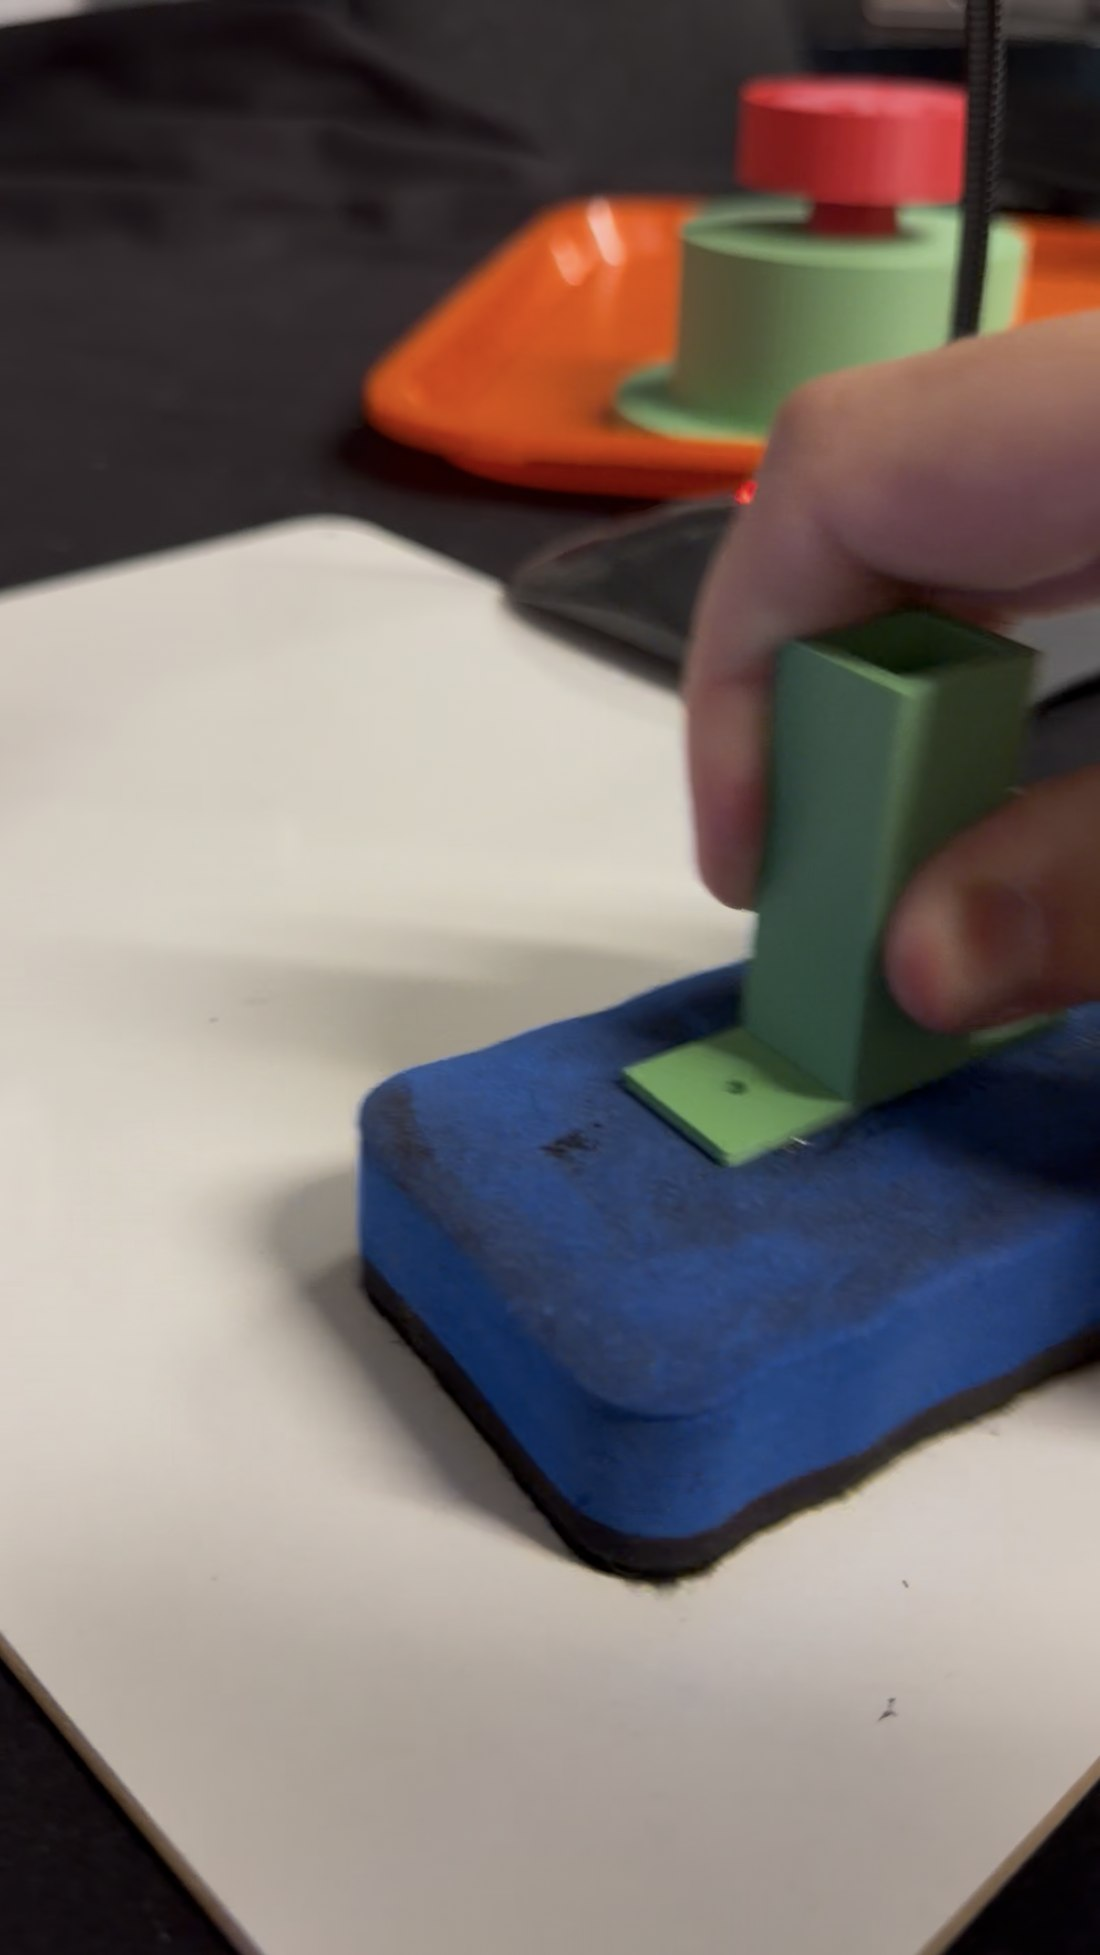
\includegraphics[height=6.5cm,keepaspectratio]{figures/task_clean.jpg}
    \caption{Cleaning the table.}
    \label{fig:task-clean}
  \end{subfigure}\hfill
  \begin{subfigure}[t]{0.31\textwidth}
    \centering
    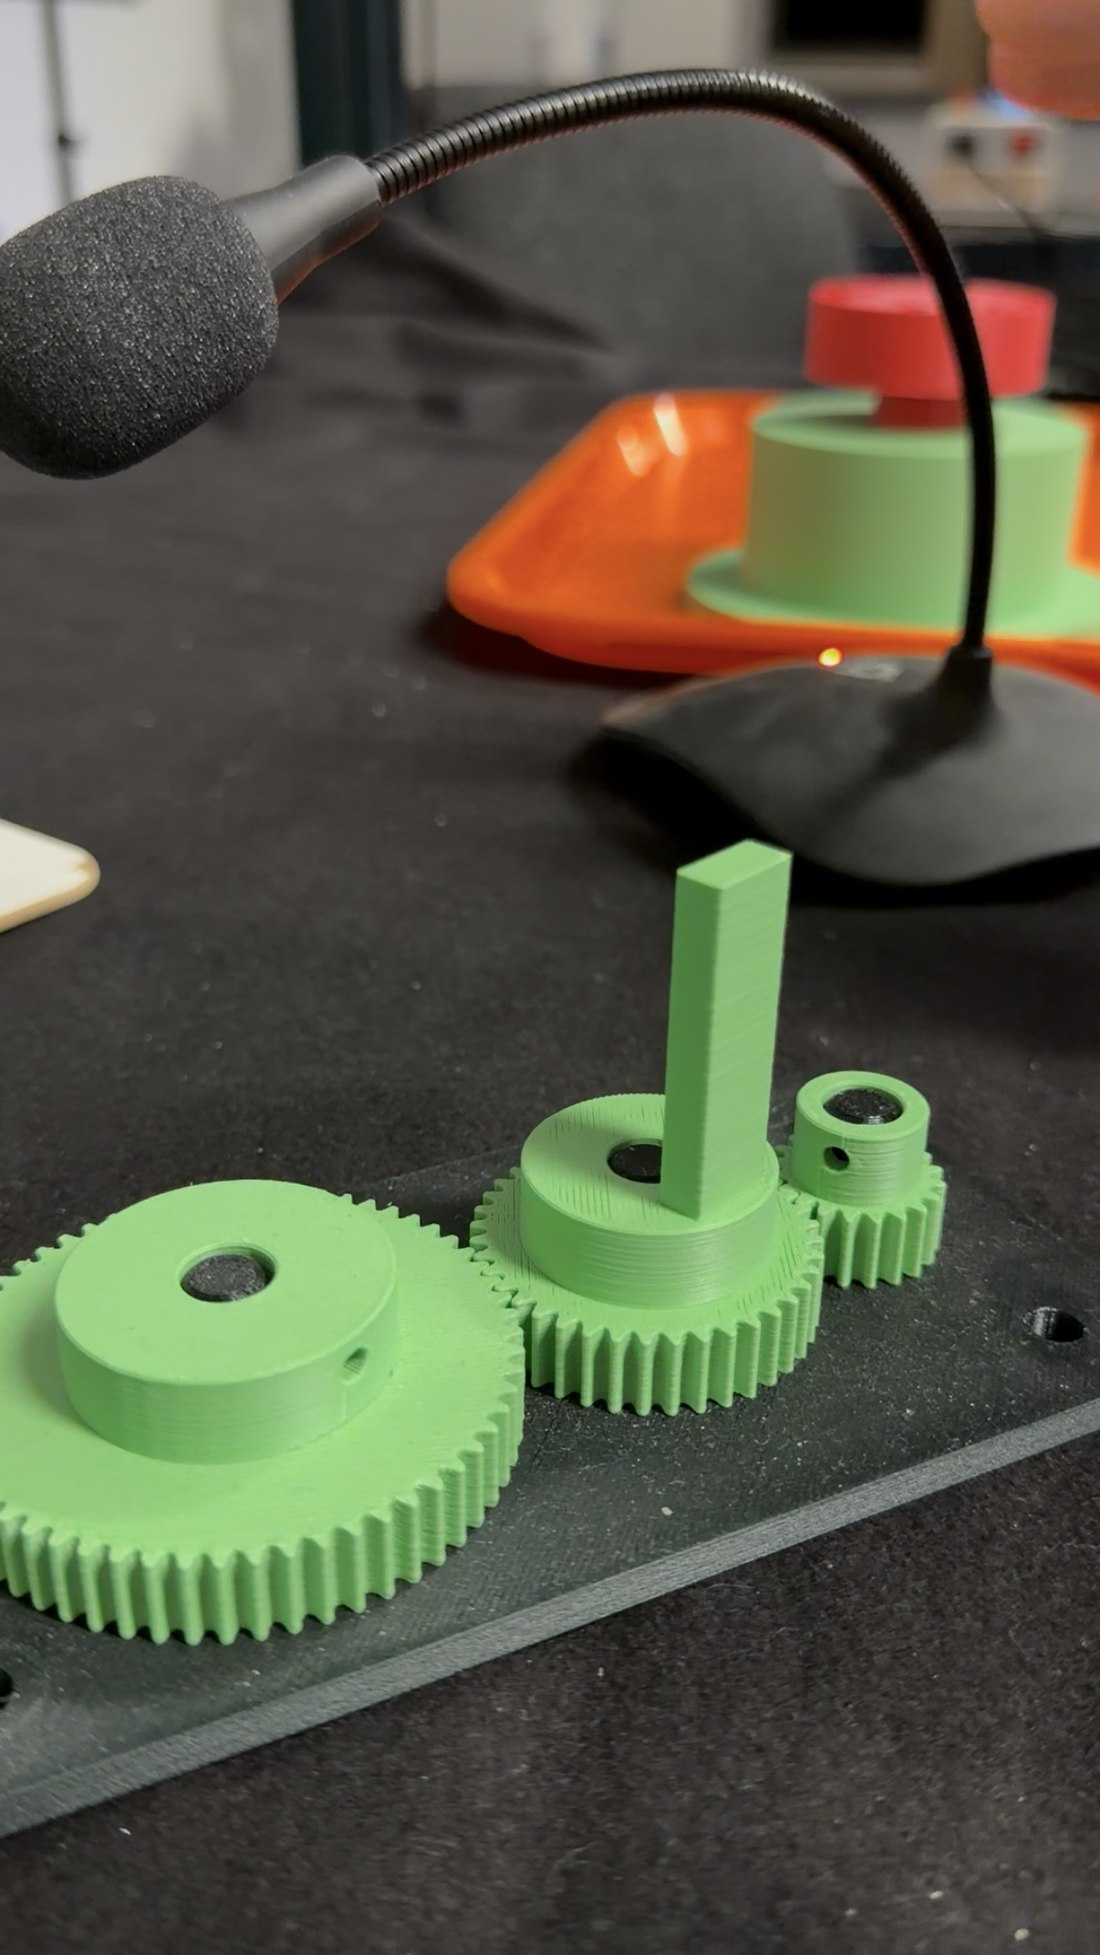
\includegraphics[height=6.5cm,keepaspectratio]{figures/task_sizes.jpg}
    \caption{Peg insertion.}
    \label{fig:task-sizes}
  \end{subfigure}\hfill
  \begin{subfigure}[t]{0.31\textwidth}
    \centering
    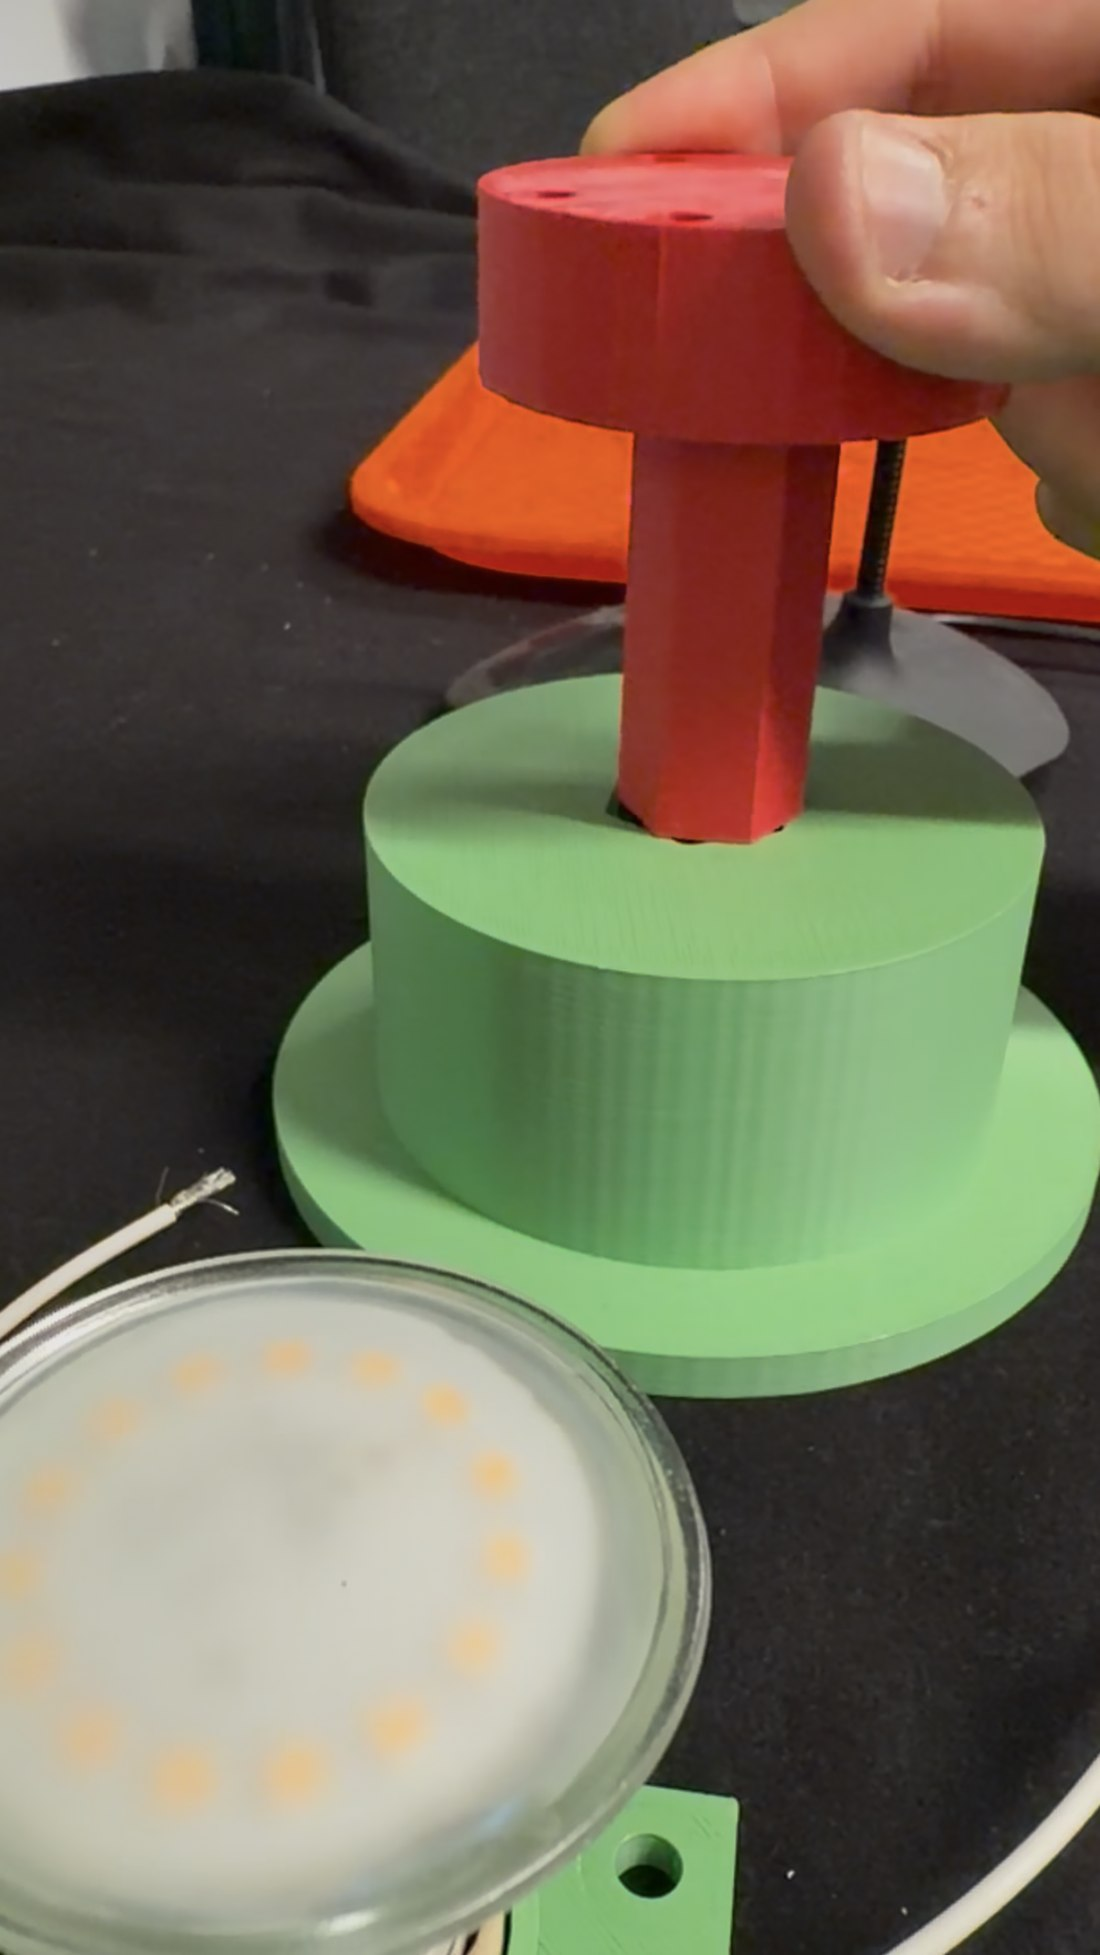
\includegraphics[height=6.5cm,keepaspectratio]{figures/task_insert.jpg}
    \caption{Peg in hole.}
    \label{fig:task-insert}
  \end{subfigure}
  \caption{The intended laboratory tasks. (a) A wiping tool pressed against the working surface. (b) Printed gears of the same shape and material but different sizes, with a peg for insertion. (c) A red peg seated into a green base. The recordings in Section~\ref{sec:results} used substitute objects.}
  \label{fig:tasks}
\end{figure}

\subsection{How the robot uses the audio}

There are two options, and the pipeline supports both. In the first, the audio is reduced to a simple signal, such as \enquote{in contact}, and a conventional controller reacts to it. In the second, the audio embedding is one input of a learned policy, next to the camera image and the robot state, as in the reviewed works. Everything up to the published spectrogram is the same in both cases, so this decision does not have to be made before recording.

\subsection{The lab session}
\label{sec:lab-measurements}

The plan was to collect demonstrations by teleoperating the Franka arm \citep{haddadin2022franka} with a SpaceMouse while audio, camera images and robot state were recorded together. With enough demonstrations, two imitation policies would be trained, one with and one without audio, and compared by task success.

This could not be done. The ROS~2 teleoperation packages were installed, but the arm could not be commanded reliably because of a configuration problem on the lab setup, and fixing it did not fit into the time of the session. Contact sounds were therefore recorded by hand using substitute objects and the same acquisition script the pipeline uses for live input. These recordings test the acquisition and representation, but they contain no joint states, no camera images and no trajectories, so no policy can be trained on them. Section~\ref{sec:results} reports what they show.

\subsection{Plan for the next session}

In the next session all streams go into one ROS~2 bag: raw audio, \topic{/audio/spectrogram}, \topic{/audio/contact_prediction}, \topic{/joint_states}, \topic{/tf}, camera images and, for teleoperation, the command topic. Raw audio is kept so that the representation or encoder can be changed later without recording again. One bag does not synchronise clocks by itself: audio and robot state should be captured on the same computer, or the clock offset must be measured. The session has three recording blocks:

\begin{enumerate}[leftmargin=*]
  \item \textbf{Robot self-noise.} The arm performs the task motion in free space without touching anything. This takes a few minutes and gives the noise that every contact sound has to rise above (Section~\ref{sec:robot-noise}). If this noise dominates, the microphone mounting or the speed must change before anything else is recorded.
  \item \textbf{Task demonstrations.} Each episode is one complete, successful execution, with the object position and start pose varied between episodes. Natural corrections, such as regaining lost contact, are kept because they teach the policy to recover.
  \item \textbf{A second surface or part}, if time allows, to see whether the results hold beyond one setup.
\end{enumerate}

The alignment script is run on every bag before the session ends, because the end of the session is the last point at which a timing problem can still be fixed with the robot available. The most important preparation is hardware: a contact microphone on the gripper (P2 in Section~\ref{sec:lit-points}).

\section{Evaluation and Results}
\label{sec:results}

Two sources of data were evaluated. The hand recordings with substitute objects (Section~\ref{sec:lab-measurements}) test acquisition, representation and whether the audio features distinguish three sound categories. Because these recordings contain no robot data, the learning step was tested on a published contact-audio dataset (Section~\ref{sec:maniwav}). The section ends with a discussion of how robot noise would change these results.

\subsection{Recording session}

The recordings used substitute objects: felt moved over paper for cleaning (\code{table_cleaning}), placement sounds made with a coin, a metal razor and a ceramic cup for the planned peg-insertion task (\code{put_sizes}), and a cup placed into a plate for the planned peg-in-hole task (\code{red_green}). The last two are sound examples for the planned tasks, not tests of actual peg insertion.

All recordings were made by hand with a USB condenser microphone, an air microphone, placed close to the contact point. Bags were written at \SI{48}{\kilo\hertz} mono in chunks of 2048 frames. Eighteen takes of 15 seconds were recorded, three per sound category and noise condition, and each was checked right after capture.

The transport layer worked in every take. All eighteen bags decode with no gaps, no overlaps and no clipped samples, and the chunk indices advance by exactly 2048 frames. The audio was reconstructed from the sample index of each chunk, so a dropout would have shown up as a hole instead of being hidden.

Figures~\ref{fig:home-panels-clean}--\ref{fig:home-panels-insert} show one take per sound category with and without noise. Wiping produces broad friction sounds, \code{put_sizes} contains separate impacts, and \code{red_green} contains placement sounds. With noise on, the events stay visible, but the background level in the spectrogram rises.

\begin{figure}[htbp]
  \centering
  \resizebox{\textwidth}{!}{\begin{tikzpicture}[x=1cm,y=1cm]

  \node[anchor=south west, font=\bfseries] at (0.00,1.05) {Cleaning: sound example --- noise off vs.\ noise on};

  \begin{axis}[
    at={(0.00cm,0cm)}, anchor=north west,
    width=6.55cm, height=2.90cm,
    xmin=0, xmax=15.00, ymin=-6457, ymax=6457,
    title={\texttt{\scriptsize table\_cleaning\_noiseoff\_01}\\[1pt]
      \scriptsize USABLE\ \textperiodcentered\ peak 5615~cts (-15.3~dBFS) \textperiodcentered\ clip $\sigma = $123.4~cts},
    title style={align=left, font=\scriptsize, at={(0,1.04)}, anchor=south west},
    ylabel={amplitude (counts)}, xlabel={}, xticklabels=\empty,
    tick label style={font=\scriptsize}, label style={font=\scriptsize},
    axis line style={black!55}, tick style={black!55},
    no markers,
  ]
    \addplot[fill=black!8, draw=none] coordinates
      {(0,-740.1) (15.00,-740.1) (15.00,740.1) (0,740.1)} -- cycle;
    \addplot[TCGreen, line width=0.2pt] table {figures/pgf/dat/table_cleaning_noiseoff_01_wave.dat};
    \node[anchor=north east, font=\tiny, text=black!45] at (rel axis cs:0.99,0.98)
      {$\pm6\sigma$ band (20\% of full scale shown)};
  \end{axis}

  \begin{axis}[
    at={(0.00cm,-3.10cm)}, anchor=north west,
    width=6.55cm, height=3.70cm,
    xmin=0, xmax=15.00, ymin=0, ymax=128,
    xlabel={time (s)}, ylabel={mel bin},
    tick label style={font=\scriptsize}, label style={font=\scriptsize},
    axis line style={black!55}, tick style={black!55},
    enlargelimits=false, no markers,
    colormap name=magma, point meta min=-68, point meta max=-30,
  ]
    \addplot graphics [xmin=0,xmax=15.00,ymin=0,ymax=128]
      {figures/pgf/heat/table_cleaning_noiseoff_01_heat.png};
    \addplot[TCGreen, line width=1.0pt, unbounded coords=jump] table {figures/pgf/dat/table_cleaning_noiseoff_01_events.dat};
    \node[anchor=north west, font=\tiny, text=white, fill=black, fill opacity=0.55,
      text opacity=1, inner sep=1.5pt] at (rel axis cs:0.01,0.98)
      {56 detected event(s)};
  \end{axis}

  \begin{axis}[
    at={(8.10cm,0cm)}, anchor=north west,
    width=6.55cm, height=2.90cm,
    xmin=0, xmax=15.00, ymin=-6325, ymax=6325,
    title={\texttt{\scriptsize table\_cleaning\_noiseon\_02}\\[1pt]
      \scriptsize USABLE\ \textperiodcentered\ peak 5500~cts (-15.5~dBFS) \textperiodcentered\ clip $\sigma = $68.7~cts},
    title style={align=left, font=\scriptsize, at={(0,1.04)}, anchor=south west},
    ylabel={}, xlabel={}, xticklabels=\empty,
    tick label style={font=\scriptsize}, label style={font=\scriptsize},
    axis line style={black!55}, tick style={black!55},
    no markers,
  ]
    \addplot[fill=black!8, draw=none] coordinates
      {(0,-412.1) (15.00,-412.1) (15.00,412.1) (0,412.1)} -- cycle;
    \addplot[TCGreen, line width=0.2pt] table {figures/pgf/dat/table_cleaning_noiseon_02_wave.dat};
    \node[anchor=north east, font=\tiny, text=black!45] at (rel axis cs:0.99,0.98)
      {$\pm6\sigma$ band (19\% of full scale shown)};
  \end{axis}

  \begin{axis}[
    at={(8.10cm,-3.10cm)}, anchor=north west,
    width=6.55cm, height=3.70cm,
    xmin=0, xmax=15.00, ymin=0, ymax=128,
    xlabel={time (s)}, ylabel={},
    tick label style={font=\scriptsize}, label style={font=\scriptsize},
    axis line style={black!55}, tick style={black!55},
    enlargelimits=false, no markers,
    colormap name=magma, point meta min=-68, point meta max=-30, colorbar, colorbar style={width=0.28cm, tick label style={font=\scriptsize}, ylabel={dB}, ylabel style={font=\scriptsize, yshift=-2mm}, ytick={-70,-60,-50,-40,-30}},
  ]
    \addplot graphics [xmin=0,xmax=15.00,ymin=0,ymax=128]
      {figures/pgf/heat/table_cleaning_noiseon_02_heat.png};
    \addplot[TCGreen, line width=1.0pt, unbounded coords=jump] table {figures/pgf/dat/table_cleaning_noiseon_02_events.dat};
    \node[anchor=north west, font=\tiny, text=white, fill=black, fill opacity=0.55,
      text opacity=1, inner sep=1.5pt] at (rel axis cs:0.01,0.98)
      {60 detected event(s)};
  \end{axis}

\end{tikzpicture}
}
  \caption{Cleaning sound example: felt on paper, noise off (left) and noise on (right). The shaded band is \(\pm6\sigma\), where \(\sigma\) is the standard deviation of the whole recording, including contact sounds. It is not the noise floor. The spectrogram uses the same filterbank settings as the live pipeline, but is computed over the whole clip without the live path's peak scaling of each one-second window.}
  \label{fig:home-panels-clean}
\end{figure}

\begin{figure}[htbp]
  \centering
  \resizebox{\textwidth}{!}{\begin{tikzpicture}[x=1cm,y=1cm]

  \node[anchor=south west, font=\bfseries] at (0.00,1.05) {Peg insertion: sound example --- noise off vs.\ noise on};

  \begin{axis}[
    at={(0.00cm,0cm)}, anchor=north west,
    width=6.55cm, height=2.90cm,
    xmin=0, xmax=15.00, ymin=-6703, ymax=6703,
    title={\texttt{\scriptsize put\_sizes\_noiseoff\_01}\\[1pt]
      \scriptsize USABLE\ \textperiodcentered\ peak 5829~cts (-15.0~dBFS) \textperiodcentered\ clip $\sigma = $293.5~cts},
    title style={align=left, font=\scriptsize, at={(0,1.04)}, anchor=south west},
    ylabel={amplitude (counts)}, xlabel={}, xticklabels=\empty,
    tick label style={font=\scriptsize}, label style={font=\scriptsize},
    axis line style={black!55}, tick style={black!55},
    no markers,
  ]
    \addplot[fill=black!8, draw=none] coordinates
      {(0,-1761.2) (15.00,-1761.2) (15.00,1761.2) (0,1761.2)} -- cycle;
    \addplot[TCBlue, line width=0.2pt] table {figures/pgf/dat/put_sizes_noiseoff_01_wave.dat};
    \node[anchor=north east, font=\tiny, text=black!45] at (rel axis cs:0.99,0.98)
      {$\pm6\sigma$ band (20\% of full scale shown)};
  \end{axis}

  \begin{axis}[
    at={(0.00cm,-3.10cm)}, anchor=north west,
    width=6.55cm, height=3.70cm,
    xmin=0, xmax=15.00, ymin=0, ymax=128,
    xlabel={time (s)}, ylabel={mel bin},
    tick label style={font=\scriptsize}, label style={font=\scriptsize},
    axis line style={black!55}, tick style={black!55},
    enlargelimits=false, no markers,
    colormap name=magma, point meta min=-68, point meta max=-30,
  ]
    \addplot graphics [xmin=0,xmax=15.00,ymin=0,ymax=128]
      {figures/pgf/heat/put_sizes_noiseoff_01_heat.png};
    \addplot[TCBlue, line width=1.0pt, unbounded coords=jump] table {figures/pgf/dat/put_sizes_noiseoff_01_events.dat};
    \node[anchor=north west, font=\tiny, text=white, fill=black, fill opacity=0.55,
      text opacity=1, inner sep=1.5pt] at (rel axis cs:0.01,0.98)
      {51 detected event(s)};
  \end{axis}

  \begin{axis}[
    at={(8.10cm,0cm)}, anchor=north west,
    width=6.55cm, height=2.90cm,
    xmin=0, xmax=15.00, ymin=-6692, ymax=6692,
    title={\texttt{\scriptsize put\_sizes\_noiseon\_01}\\[1pt]
      \scriptsize USABLE\ \textperiodcentered\ peak 5819~cts (-15.0~dBFS) \textperiodcentered\ clip $\sigma = $315.6~cts},
    title style={align=left, font=\scriptsize, at={(0,1.04)}, anchor=south west},
    ylabel={}, xlabel={}, xticklabels=\empty,
    tick label style={font=\scriptsize}, label style={font=\scriptsize},
    axis line style={black!55}, tick style={black!55},
    no markers,
  ]
    \addplot[fill=black!8, draw=none] coordinates
      {(0,-1893.3) (15.00,-1893.3) (15.00,1893.3) (0,1893.3)} -- cycle;
    \addplot[TCBlue, line width=0.2pt] table {figures/pgf/dat/put_sizes_noiseon_01_wave.dat};
    \node[anchor=north east, font=\tiny, text=black!45] at (rel axis cs:0.99,0.98)
      {$\pm6\sigma$ band (20\% of full scale shown)};
  \end{axis}

  \begin{axis}[
    at={(8.10cm,-3.10cm)}, anchor=north west,
    width=6.55cm, height=3.70cm,
    xmin=0, xmax=15.00, ymin=0, ymax=128,
    xlabel={time (s)}, ylabel={},
    tick label style={font=\scriptsize}, label style={font=\scriptsize},
    axis line style={black!55}, tick style={black!55},
    enlargelimits=false, no markers,
    colormap name=magma, point meta min=-68, point meta max=-30, colorbar, colorbar style={width=0.28cm, tick label style={font=\scriptsize}, ylabel={dB}, ylabel style={font=\scriptsize, yshift=-2mm}, ytick={-70,-60,-50,-40,-30}},
  ]
    \addplot graphics [xmin=0,xmax=15.00,ymin=0,ymax=128]
      {figures/pgf/heat/put_sizes_noiseon_01_heat.png};
    \addplot[TCBlue, line width=1.0pt, unbounded coords=jump] table {figures/pgf/dat/put_sizes_noiseon_01_events.dat};
    \node[anchor=north west, font=\tiny, text=white, fill=black, fill opacity=0.55,
      text opacity=1, inner sep=1.5pt] at (rel axis cs:0.01,0.98)
      {23 detected event(s)};
  \end{axis}

\end{tikzpicture}
}
  \caption{Placement sounds for the planned peg-insertion task (\code{put_sizes}), noise off (left) and noise on (right). The waveform band and spectrogram follow Figure~\ref{fig:home-panels-clean}.}
  \label{fig:home-panels-sizes}
\end{figure}

\begin{figure}[htbp]
  \centering
  \resizebox{\textwidth}{!}{\begin{tikzpicture}[x=1cm,y=1cm]

  \node[anchor=south west, font=\bfseries] at (0.00,1.05) {Peg in hole: sound example --- noise off vs.\ noise on};

  \begin{axis}[
    at={(0.00cm,0cm)}, anchor=north west,
    width=6.55cm, height=2.90cm,
    xmin=0, xmax=15.00, ymin=-6829, ymax=6829,
    title={\texttt{\scriptsize red\_green\_noiseoff\_01}\\[1pt]
      \scriptsize USABLE\ \textperiodcentered\ peak 5938~cts (-14.8~dBFS) \textperiodcentered\ clip $\sigma = $267.3~cts},
    title style={align=left, font=\scriptsize, at={(0,1.04)}, anchor=south west},
    ylabel={amplitude (counts)}, xlabel={}, xticklabels=\empty,
    tick label style={font=\scriptsize}, label style={font=\scriptsize},
    axis line style={black!55}, tick style={black!55},
    no markers,
  ]
    \addplot[fill=black!8, draw=none] coordinates
      {(0,-1603.6) (15.00,-1603.6) (15.00,1603.6) (0,1603.6)} -- cycle;
    \addplot[TCOrange, line width=0.2pt] table {figures/pgf/dat/red_green_noiseoff_01_wave.dat};
    \node[anchor=north east, font=\tiny, text=black!45] at (rel axis cs:0.99,0.98)
      {$\pm6\sigma$ band (21\% of full scale shown)};
  \end{axis}

  \begin{axis}[
    at={(0.00cm,-3.10cm)}, anchor=north west,
    width=6.55cm, height=3.70cm,
    xmin=0, xmax=15.00, ymin=0, ymax=128,
    xlabel={time (s)}, ylabel={mel bin},
    tick label style={font=\scriptsize}, label style={font=\scriptsize},
    axis line style={black!55}, tick style={black!55},
    enlargelimits=false, no markers,
    colormap name=magma, point meta min=-68, point meta max=-30,
  ]
    \addplot graphics [xmin=0,xmax=15.00,ymin=0,ymax=128]
      {figures/pgf/heat/red_green_noiseoff_01_heat.png};
    \addplot[TCOrange, line width=1.0pt, unbounded coords=jump] table {figures/pgf/dat/red_green_noiseoff_01_events.dat};
    \node[anchor=north west, font=\tiny, text=white, fill=black, fill opacity=0.55,
      text opacity=1, inner sep=1.5pt] at (rel axis cs:0.01,0.98)
      {8 detected event(s)};
  \end{axis}

  \begin{axis}[
    at={(8.10cm,0cm)}, anchor=north west,
    width=6.55cm, height=2.90cm,
    xmin=0, xmax=15.00, ymin=-6979, ymax=6979,
    title={\texttt{\scriptsize red\_green\_noiseon\_01}\\[1pt]
      \scriptsize USABLE\ \textperiodcentered\ peak 6069~cts (-14.6~dBFS) \textperiodcentered\ clip $\sigma = $482.5~cts},
    title style={align=left, font=\scriptsize, at={(0,1.04)}, anchor=south west},
    ylabel={}, xlabel={}, xticklabels=\empty,
    tick label style={font=\scriptsize}, label style={font=\scriptsize},
    axis line style={black!55}, tick style={black!55},
    no markers,
  ]
    \addplot[fill=black!8, draw=none] coordinates
      {(0,-2894.8) (15.00,-2894.8) (15.00,2894.8) (0,2894.8)} -- cycle;
    \addplot[TCOrange, line width=0.2pt] table {figures/pgf/dat/red_green_noiseon_01_wave.dat};
    \node[anchor=north east, font=\tiny, text=black!45] at (rel axis cs:0.99,0.98)
      {$\pm6\sigma$ band (21\% of full scale shown)};
  \end{axis}

  \begin{axis}[
    at={(8.10cm,-3.10cm)}, anchor=north west,
    width=6.55cm, height=3.70cm,
    xmin=0, xmax=15.00, ymin=0, ymax=128,
    xlabel={time (s)}, ylabel={},
    tick label style={font=\scriptsize}, label style={font=\scriptsize},
    axis line style={black!55}, tick style={black!55},
    enlargelimits=false, no markers,
    colormap name=magma, point meta min=-68, point meta max=-30, colorbar, colorbar style={width=0.28cm, tick label style={font=\scriptsize}, ylabel={dB}, ylabel style={font=\scriptsize, yshift=-2mm}, ytick={-70,-60,-50,-40,-30}},
  ]
    \addplot graphics [xmin=0,xmax=15.00,ymin=0,ymax=128]
      {figures/pgf/heat/red_green_noiseon_01_heat.png};
    \addplot[TCOrange, line width=1.0pt, unbounded coords=jump] table {figures/pgf/dat/red_green_noiseon_01_events.dat};
    \node[anchor=north west, font=\tiny, text=white, fill=black, fill opacity=0.55,
      text opacity=1, inner sep=1.5pt] at (rel axis cs:0.01,0.98)
      {26 detected event(s)};
  \end{axis}

\end{tikzpicture}
}
  \caption{Cup-into-plate sounds for the planned peg-in-hole task (\code{red_green}), noise off (left) and noise on (right). The waveform band and spectrogram follow Figure~\ref{fig:home-panels-clean}.}
  \label{fig:home-panels-insert}
\end{figure}

\subsection{The noise condition}
\label{sec:noise-condition}

Two reference takes without any contact were recorded, one with the noise source off and one with it on. The noise source raises the RMS level by \SI{22.2}{\decibel}, from \SI{-69.7}{} to \SI{-47.5}{dBFS}, and the estimated noise floor by \SI{6.4}{\decibel}. This floor is the median RMS level of the quietest \SI{20}{\percent} of frames. The mean event-to-floor ratio is lower under added noise in all three sound categories. The event marks in Figures~\ref{fig:home-panels-clean}--\ref{fig:home-panels-insert} show runs of at least three frames more than \SI{6}{\decibel} above this floor; they are detected sound events, not labelled contacts.

The added noise, broadband noise played from a phone loudspeaker, is not the same as the noise of the Franka arm. Its spectrum differs, and it reaches the microphone through the air, while motor noise mostly travels through the arm into the tool. This experiment therefore measures robustness to one ambient noise at a known level, not to robot noise. Section~\ref{sec:robot-noise} discusses the difference.

\subsection{Can the audio features tell the sounds apart?}
\label{sec:separation}

Features were computed with the pipeline's own spectrogram code: \SI{1.0}{\second} windows every \SI{0.5}{\second}, each giving a \(98\times128\) filterbank, which was checked by assertion. The three encoder bundles of the ML node produced the embeddings.

The classifier uses cosine nearest-centroid matching: it compares each window's features with the average features of each sound category from the other clips. The category with the most window votes becomes the clip prediction. This is repeated with each clip held out once (leave-one-clip-out). The chance level is estimated from 2,000 shuffles of the labels between clips. Clips, not windows, are the unit, because overlapping windows from the same recording are not independent. A random split of windows would put parts of the same recording into training and test data and overestimate the accuracy.

\begin{table}[htbp]
  \centering
  \caption{Separation of the three sound categories by encoder. Per-clip: correctly classified clips. \(p\): fraction of label shuffles with accuracy at least as high as the measured result, rounded to three decimals.}
  \label{tab:separability}
  \begin{tabular}{lrrr}
    \toprule
    Encoder & Silhouette & Per-clip & \(p\) \\
    \midrule
    \code{cnn}      & \num{+0.057} & 9/18  & 0.164 \\
    \code{melstats} & \num{+0.047} & 10/18 & 0.090 \\
    \code{ast}      & \num{+0.063} & \textbf{15/18} & \textbf{0.001} \\
    \bottomrule
  \end{tabular}
\end{table}

The classifier using AST features gets 15 of 18 clips right (\(p\approx\num{0.001}\)); the CNN and mel-statistics results are not clearly above chance (\(p=0.164\) and \(p=0.090\)). The AST-feature classifier gets all \code{table_cleaning} and \code{put_sizes} takes right, and all quiet \code{red_green} takes. Its three errors are the noisy \code{red_green} takes, all predicted as \code{put_sizes}. Both categories contain placement sounds, so noise may hide a useful cue. Material and recording differences could also explain the confusion. Figure~\ref{fig:home-embedding} shows the embeddings.

\begin{figure}[htbp]
  \centering
  % Keep the original scatter plots. Typeset readable, corrected labels in LaTeX.
% The 4050 x 1440 pixel source is 300 dpi. Trim only its old titles and legend.
\begin{minipage}[t]{0.32\textwidth}
  \centering\sffamily\small
  \textbf{CNN}\\
  9/18 correct; \(p=0.164\)
\end{minipage}\hfill
\begin{minipage}[t]{0.32\textwidth}
  \centering\sffamily\small
  \textbf{Mel statistics}\\
  10/18 correct; \(p=0.090\)
\end{minipage}\hfill
\begin{minipage}[t]{0.32\textwidth}
  \centering\sffamily\small
  \textbf{AST}\\
  15/18 correct; \(p\approx0.001\)
\end{minipage}
\par\smallskip
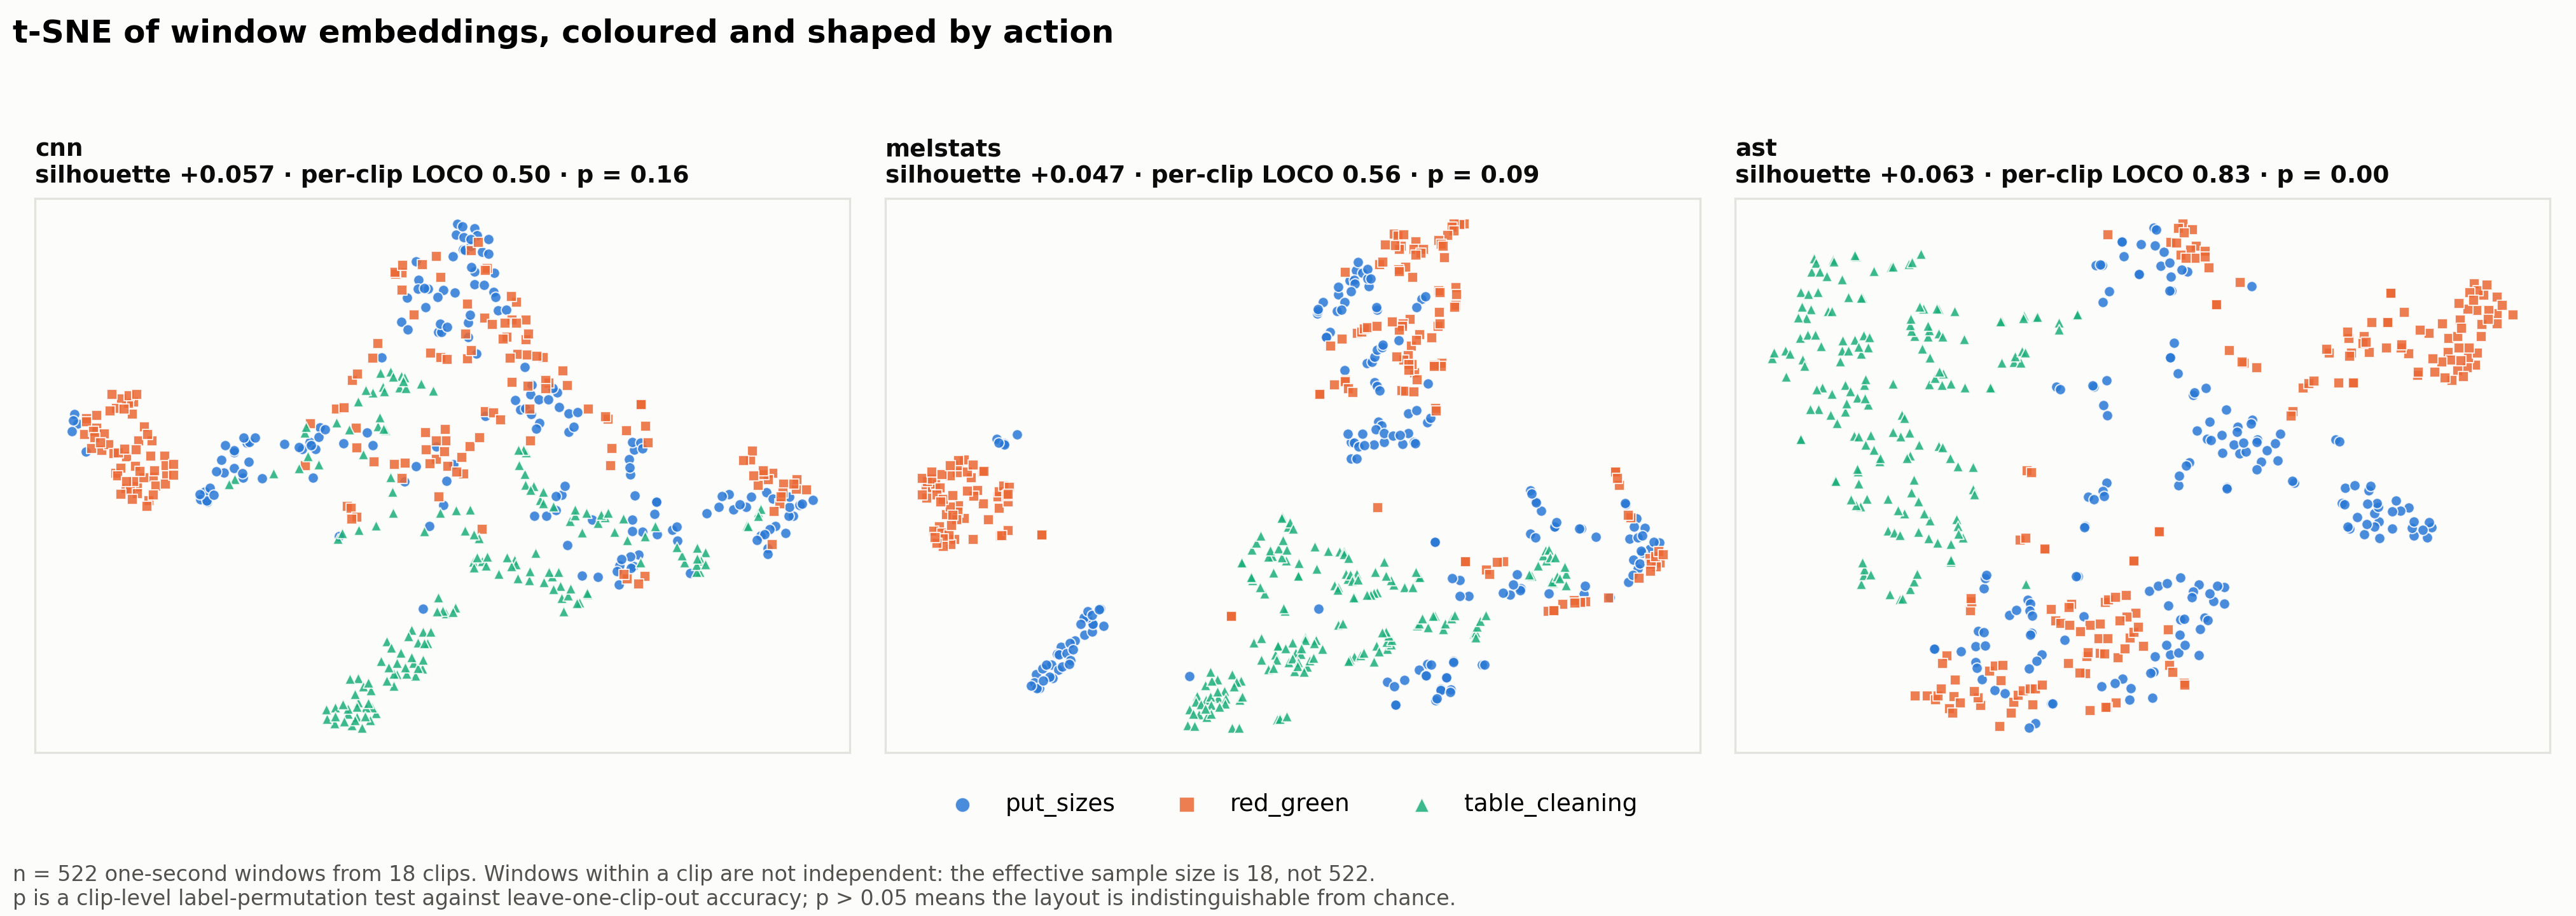
\includegraphics[width=\textwidth,trim=0bp 57.6bp 0bp 72bp,clip]{figures/home_embedding.png}
\par\smallskip
{\small
  \tikz[baseline=-0.5ex]{\fill[TCBlue] (0,0) circle (1.5pt);}\ \code{put_sizes}
  \qquad
  \tikz[baseline=-0.5ex]{\fill[TCOrange] (0,0) rectangle (3pt,3pt);}\ \code{red_green}
  \qquad
  \tikz[baseline=-0.5ex]{\fill[TCGreen] (0,0) -- (3.5pt,0) -- (1.75pt,3.5pt) -- cycle;}\ \code{table_cleaning}
}

  \caption{t-SNE \citep{vandermaaten2008tsne} view of 522 window embeddings from 18 clips. Colour and marker shape show the sound category. The accuracy and \(p\)-values come from the clip-level test in Table~\ref{tab:separability}, not from the positions in this plot.}
  \label{fig:home-embedding}
\end{figure}

The result has clear limits. It is one dataset of eighteen clips, so it does not rank the encoders in general. The objects also differ in material, so the classifier may recognise materials as well as actions. It has not been tested on real peg insertion.

\subsection{Testing the learning step on ManiWAV}
\label{sec:maniwav}

\paragraph{Why this experiment.} The recordings from this project lack camera images and pose data, so they cannot provide actions for policy training. To test the learning step, the released \code{wipe} dataset of ManiWAV \citep{liu2024maniwav} was used. It was recorded with a contact microphone in a handheld UMI gripper and is close to the planned cleaning task. The question is: \emph{can audio features predict the next motion, and do they help when the current pose and gripper width are already known?}

\paragraph{Setup.} The pipeline produced \num{16565} AST embeddings from 78 episodes at \SI{15}{\hertz}, using the same \(98\times128\) spectrograms as before. The audio input contains 30 overlapping one-second windows. Their endpoints span about two seconds, while the audio itself spans about \SI{2.93}{\second}. The pose input contains only the current position, orientation and gripper width; it has no pose history or speed input.

The targets use the ten-value layout described in Section~\ref{sec:policy-data}: 16 consecutive pose changes and the next gripper widths. At the assumed \SI{60}{\hertz} data rate, these cover about \SI{0.27}{\second}. ManiWAV's released setup instead samples action steps at about \SI{20}{\hertz} and expresses future poses relative to the current observation pose. A small network was trained with current pose and gripper width only, audio only, or both. Eight random splits each held out 16 of the 78 episodes.

The error is mean squared error (MSE) after each action value is centred and scaled to unit standard deviation. These means and scales, for both inputs and targets, were computed from all episodes before splitting. The constant baseline predicts the full-dataset mean action. Each learned model reports its lowest validation error over 40 epochs. This lets validation data affect preprocessing and model selection, so the scores are early checks, not results on an independent test set.

\begin{table}[htbp]
  \centering
  \caption{Early action-prediction test on ManiWAV \code{wipe}: MSE on standardised action targets, mean and sample standard deviation over eight splits. Lower is better. Scaling uses all episodes; model scores use the best validation epoch.}
  \label{tab:maniwav}
  \begin{tabular}{lrr}
    \toprule
    Input & Validation MSE & Change from baseline \\
    \midrule
    Full-dataset mean action & \num{1.0179} \(\pm\) \num{0.0695} & --- \\
    Current pose and gripper width & \num{0.7383} \(\pm\) \num{0.0525} & \SI{-27.5}{\percent} \\
    Audio only             & \num{0.8088} \(\pm\) \num{0.0687} & \SI{-20.5}{\percent} \\
    Audio, current pose and gripper width & \num{0.7309} \(\pm\) \num{0.0616} & \SI{-28.2}{\percent} \\
    \bottomrule
  \end{tabular}
\end{table}

\paragraph{Result.} Audio alone gives \SI{20.5}{\percent} lower mean validation MSE than the constant baseline and beats it in all eight splits. It has higher error than the pose-and-gripper input in all eight splits. Adding audio to that input lowers the mean error by about \SI{1}{\percent}, with improvement in five of eight splits. The paired error reduction is \num{0.0074} \(\pm\) \num{0.0162} (mean and sample standard deviation). This suggests that audio carries some information about motion, but its added value beside the current pose and gripper width remains unclear. Sound may also reflect wiping speed; this test does not show which cues the network uses.

\paragraph{Limitations.} This test uses a frozen encoder, no images, 78 of the 119 released episodes and a small network instead of a diffusion policy. It measures prediction error, not task success, and does not reproduce ManiWAV. A stronger test needs scaling and a mean baseline computed from training episodes only, plus a separate test set. The eight splits share episodes, so their spread is not a significance test. The \SI{60}{\hertz} data rate and the choice of \code{mic_0} were inferred from the data during this run and still need checking against the source recording details.

\subsection{How robot noise would affect the audio and policy learning}
\label{sec:robot-noise}

On the robot, the main noise source is the robot itself. The joint motors and gearboxes, the brakes, the gripper and the cooling fans of the controller all produce sound and vibration. This noise affects the sensor readings in three ways.

\begin{enumerate}[leftmargin=*]
  \item \textbf{It raises the noise floor.} As with the loudspeaker (Section~\ref{sec:noise-condition}), weak contact sounds such as light wiping or slow sliding can sink below the floor, and in the spectrogram the whole image becomes brighter. With a contact microphone on the gripper this effect is likely much stronger than with an air microphone, because motor vibration travels through the links into the gripper along the same path as the contact signal.
  \item \textbf{It changes with the motion.} Unlike the constant loudspeaker noise, motor noise appears when the arm moves and disappears when it stops, and its level and frequency depend on joint speed and acceleration. In the spectrogram it appears as bands that follow the trajectory.
  \item \textbf{It differs between data collection and deployment.} If demonstrations are recorded with a handheld gripper, as in UMI and ManiWAV, there is no motor noise in the training audio, but there is on the robot. ManiWAV names nonlinear motor noise as one of the two main reasons for this gap, next to unexpected sounds from the robot's own interactions \citep{liu2024maniwav}.
\end{enumerate}

For policy learning, each of these has a consequence. Masking removes contact cues, so the audio branch contributes less and the policy relies on vision and pose again. Motion-dependent noise creates a shortcut: a policy may learn the robot's speed from its sound instead of learning about contact, and then fail when the speed changes. A pose history can also provide motion information, but the test in Section~\ref{sec:maniwav} used only the current pose and does not establish this shortcut. Finally, new sounds during deployment can change the encoder's features and therefore the actions. ManiWAV reduces this gap by recording ten samples of motor noise on the robot and mixing them, together with ESC-50 background sounds, into the training audio; this worked better than filtering the noise at test time \citep{liu2024maniwav}.

For this project, teleoperating the Franka arm means the motor noise is already in the demonstrations, so the gap in point~3 is small, but the shortcut remains. Four measures follow from this: record the self-noise block first (Section~\ref{sec:plan}); mount the contact microphone with damping and away from the motors; add recorded robot noise to the training audio; and check that the audio features of free-space motion differ from those of contact, so that the policy reacts to contact and not only to motion.

\subsection{What the results show}

The results show that the pipeline works on real audio: eighteen recordings arrive without gaps, the \(98\times128\) representation holds for the project's recordings and for an external dataset, and the alignment logic detects timing errors in simulation. The AST-feature classifier identifies the three sound categories in 15 of 18 clips, with all errors under added noise. In the early test on contact-microphone data, audio features give lower validation error than a constant baseline. RQ2 is partly answered; live recording with a contact microphone and timing against the real robot still need testing. RQ1 remains open: the planned robot study must test whether audio improves task success beyond vision and pose.

The session also improved the recording procedure. Checking each take right after recording caught four bad takes (a cough, two takes in which the noise did not reach the microphone, and one take \SI{27}{\decibel} too quiet), which were recorded again on the spot. A level check before each take (tap the tool, require a peak of at least \SI{-20}{dBFS}, reject clipping) should be added to the recording script. A thirty-second reference recording without contact turns the noise level from an assumption into a measurement.

\section{Conclusion and Outlook}
\label{sec:conclusion}

This project built the audio software needed for a robot to listen to its contacts. A ROS~2 pipeline records audio, turns it into a documented spectrogram, encodes it with a choice of models, and provides time-stamped features. Offline scripts match these features with poses and build action chunks. First results are promising: a classifier using pretrained audio features separates three sound categories recorded with an air microphone and substitute objects. An early test on a published contact-microphone dataset also suggests that the features contain information about motion.

The next steps follow directly from the literature and from these results:

\begin{enumerate}[leftmargin=*]
  \item mount a piezoelectric contact microphone on the gripper of the Franka arm and measure the robot's self-noise;
  \item record teleoperated demonstrations of cleaning the table and of peg insertion, with audio, camera and robot state in one synchronised bag;
  \item train a policy, such as Diffusion Policy, with and without audio, using recorded robot noise as augmentation;
  \item compare task success on the real robot, focusing on the moments where contact is made, lost or completed.
\end{enumerate}

With the software in place, these steps need mainly robot time and a contact microphone, and they would answer the question this project started with: does a robot manipulate better when it can hear?

\bibliographystyle{plainnat}
\bibliography{references}

\end{document}
